%!TEX root = ../dokumentation.tex

% Dokumentieren Sie Ihre Ergebnisse mit 2-3 Seiten (inkl. Bilder). Gehen Sie
% insbesondere auf die Ermittlung der möglichen Züge, ihre Bewertungsfunktion
% und die Schwierigkeitsgrade ein. Zeigen Sie Ihre KI in interessanten Situationen
% (gut oder schlecht). Formulieren Sie einen „KI-Trick“ wie die in der Vorlesung
% gezeigten mit dem aus Ihrer Sicht interessantesten Aspekt ihrer KI. 
% Gehen Sie darauf ein, wie Sie ihre KI getestet und iteriert haben.

\chapter{Evaluation}

Insgesamt kann man sagen, dass die KI eine gut Spielstärke aufweist. Sie besiegt in allen Ausgangssituation die vorgegeben Greedy-KI, egal ob auf der startenden Seite oder auch nicht. Auch gegen einen echten Gegner stellt sie sich gut an und kann diesen besiegen. 

\subsubsection{Bewertungsfunktionen}

Die Bewertungsfunktion der Angriffe funktioniert im Großen und Ganzen sehr gut. Es werden die stärkeren Gegner zuerst angegriffen. Die Überprüfung ob man eine Einheit töten kann ermöglicht es schnell viele Schaden durch den Gegner abzuwenden. Durch die verwendete Hierarchie kommt es häufig zu Situationen in denen relativ schnell die starken Einheiten des Gegners getötet wurden. Auch Siege in denen Czaremir stirbt und einige Einheiten zurücklässt treten nicht selten auf. Eine weitere gut funktionierende Bewertung findet für das Angreifen gegnerischer Bummz statt, diese werden bei ungünstigen Feldern nur sehr selten angegriffen, bei vorteilhaften Positionierungen lassen sich gezielte Angriffe und der daraus entstehende Flächenschaden sehr gut erkennen. 

\begin{figure}[H]
	\begin{minipage}[b]{.4\linewidth} % [b] => Ausrichtung an \caption
		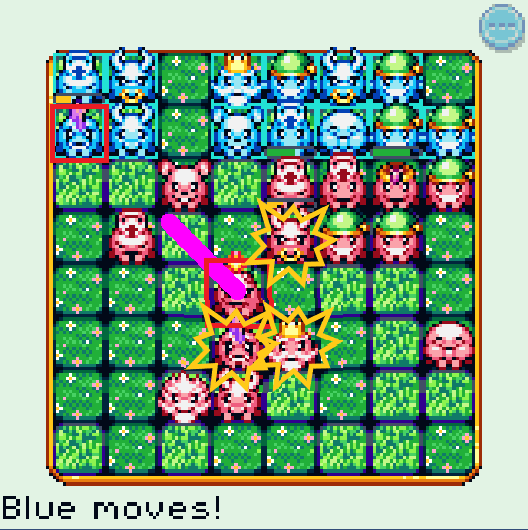
\includegraphics[width=\linewidth]{bummz}
		\caption{Angriff auf Bummz schadet wichtigen Einheiten}
	\end{minipage}
	\hspace{.1\linewidth}% Abstand zwischen Bilder
	\begin{minipage}[b]{.4\linewidth} % [b] => Ausrichtung an \caption
		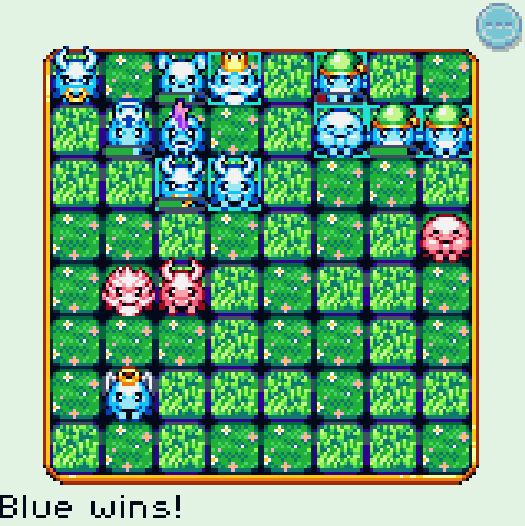
\includegraphics[width=\linewidth]{koenigtot}
		\caption{Spiel wird durch das Töten des Königs gewonnen}
	\end{minipage}
\end{figure}

Verbesserungen für die Angriffsbewertung könnten bei der Vergabe der Zahlenwerte angesetzt werden. Diese sind nur grundlegend an die Erkenntnisse der vorhandenen Spielstände angepasst und könnten durch weitere Spielsituationen und Analysen verbessert werden. An dieser Stelle könnte man auch die Konstanten durch Funktionen wie sie bei Bummz, Haley, Buffy und Link zu finden sind für weitere Einheiten ersetzen. Dies würde eine dynamischere Bewertung von Angriffen ermöglichen und so auch bei verschiedenen Spielsituationen eine passende Angriffsentscheidung ermöglichen. Ein Beispiel dafür wäre das allgemein aggressivere Spielen sollte man sich in Führung befinden. Zuletzt könnten einzelne Comparer für jede Einheit geschrieben werden, welche es der KI ermöglicht beispielsweise einen Fokus auf eine ganz bestimmte Einheit zu legen. 
% allgemeine Bewertung/Zahlen anpassen, Funktionen für Units entwickeln, Spielstatus abhängige Entscheidungen, verschiedene AttackComparer für unterschiedliche Units (Fokus setzen)

Die Bewertungsfunktion der Bewegung ist insgesamt gut gelungen und bildet eine starke Grundlage. Sehr bewegliche Einheiten mit großer Reichweite halten sich schön entfernt und greifen aus großer Distanz an, weshalb sie selten ein Ziel der Gegner sind. Auch die Bewegung der Tanks stellt dafür eine gute Absicherung dar. Außerdem lässt sich sehr oft eine durchdachte Gesamtaufstellung erkennen, welche strukturiert Richtung Gegner zieht. 

\begin{figure}[H]
	\begin{minipage}[b]{.4\linewidth} % [b] => Ausrichtung an \caption
		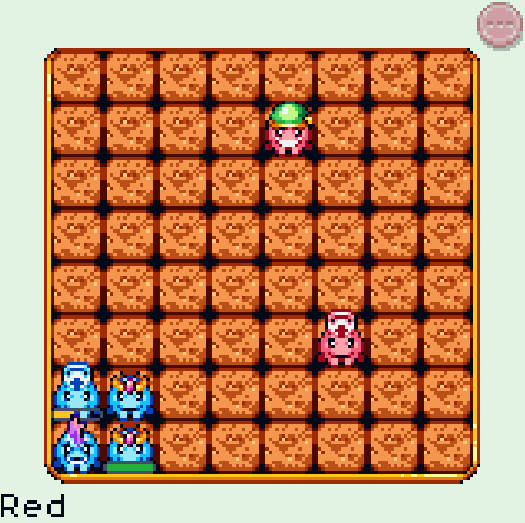
\includegraphics[width=\linewidth]{schlechteposi}
		\caption{Flächeneffekte zu hoch bewertet - Sneip kann nicht aus seiner Ecke}
	\end{minipage}
	\hspace{.1\linewidth}% Abstand zwischen Bilder
	\begin{minipage}[b]{.4\linewidth} % [b] => Ausrichtung an \caption
		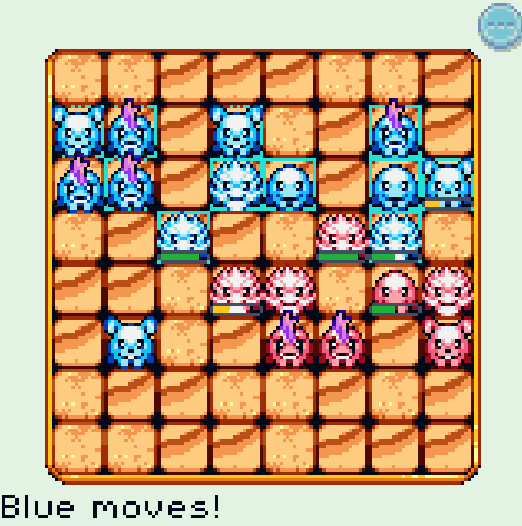
\includegraphics[width=\linewidth]{guteposi}
		\caption{Alle Sneips haben Ziel und keine Angreifer - Tanks an der Front}
	\end{minipage}
\end{figure}

Dennoch können Spielsituationen in denen strategisch schlechte Züge ausgeführt werden nicht vollständig vermieden werden. Auch hier wäre eine Bewertung der Bewegung je nach Spielsituation hilfreich. So kann beispielsweise bei Führung eine aggressive Vorwärtsbewegung ausgeführt werden oder auch der König bei wenig übrigen Einheiten aktiviert werden, um sein Schaden auszunutzen anstatt passiv zu spielen. Außerdem kommt es in Spielsituationen mit vielen Einheiten dazu, dass diese sich gegenseitig blockieren und theoretisch möglicher Schaden oder bessere Positionen verloren gehen. Zudem könnte man die Bewegungsbewertung besser aufteilen, sodass jede Einheit seine eigene Bewertungsfunktion erhält und diese so perfekt auf die Eigenschaften dieser zugeschnitten ist. Hier könnte man dann ebenfalls ein gezielteres Bewegen einführen, welches zum Beispiel stärker Richtung gegnerischem Czaremir orientiert ist, um diesen schneller zu töten. Zuletzt könnte die Bewegung einer Einheit abhängig von dessen momentanen Eigenschaften umgesetzt werden. Hat eine Einheit mehr Angriffskraft oder weniger Lebenspunkt als zuvor, dann ändert sie ihre Bewegung im Bezug auf Aggressivität. 

% mehr Unit-Abhängigkeit,  gezielter Laufen (zum König), Bewegung abhängig von HP

\subsubsection{Der KI-Trick}

Kombinieren der Angriffskraft vieler einzelner Einheiten, um einen starken Angriff auf einen einzelnen Gegner durchzuführen. Es wird für jede Einheit geschaut, ob mit Hilfe dieser eine andere Einheit noch im selben Zug getötet werden kann. Dadurch ist es möglich seinen Angriff zu sammeln und schnell Einheiten des Gegners zu töten, sodass diese den eigenen Einheiten keinen Schaden mehr zufügen können, also der Gesamtschaden, der auszuhalten ist, reduziert wird.

\subsubsection{Testen und Iterieren}

Zum Testen und Iterieren der KI wurde wie folgt vorgegangen. Es wurden die einzelnen verfügbaren Startsituationen durchgespielt, wobei der Fokus auf der zuletzt veränderten Einheit lag. Hierbei wurde Schritt für Schritt jede Bewegung und Angriff der Einheit angeschaut und nachvollzogen. Bei Auffälligkeiten oder strategisch schlechten Zügen wurden die Parameter des jeweiligen Zeitpunkts genauer analysiert und im Notfall die exakten Bewertungen berechnet. Anhand der Erkenntnisse wurden dann die Parameter der Bewertung angepasst. Das Erstellen eines neuen DecisionTrees baut auf den DecisionTrees anderer Einheiten sowie der im Konzept überlegten strategischen Grundlagen auf.

% verschiedene Spielsituationen ausgewählt, Fokus auf veränderte Einheit, bei Auffälligkeiten Debug und Nachrechnen,

% Bummz anpassen: genaue Berechnung was passiert, wenn sie an den möglichen Felder auf die sie sich bewegt, stirbt
% Unterscheidung zwischen Unit die wir töten und Units die wir nicht töten können (wegen Chilly)
% keine Spielstand abhängigen Entscheidungen